\documentclass[tikz]{standalone}
\usepackage{fontspec}
\renewcommand*{\familydefault}{\sfdefault}
\usepackage{standalone}
%\usetikzlibrary{arrows.meta, decorations.pathreplacing, shapes.geometric}
\usetikzlibrary{bayesnet}

\begin{document}

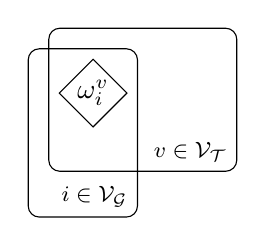
\begin{tikzpicture}

% Define nodes
\path (0,0)
node[det] (omega) {\(\omega^v_i\)}
%to
%(180:2.5 cm)
%node[latent] (U) {\(\mathbf{U}^\mathrm{sel}\)}
(omega) +(1.7,0.7) coordinate (tree)
(omega) +(-0.7,-1) coordinate (site)
;

% Plates
\plate {Xtree} {(omega) (tree)} {\(v\in\mathcal{V}_\mathcal{T}\)} ;
\plate {Xsite} {(omega) (site)} {\(i\in\mathcal{V}_\mathcal{G}\)} ;


\end{tikzpicture}

\end{document}
